
\section[Parallel Speedup]{Parallel Speedup}
\label{sec:speedup}
\addcontentsline{toc}{section}{\thesection. Parallel Speedup}

The main bottleneck of \pkg{cubfits} is in calls to \code{fitMultinom*()} or
\code{my.fitMultinom*()}. The reasons are that
\begin{itemize}
\item models assume conditional independence of amino acids, and
\item it is tedious to extract parallelism within the 
\code{VGAM::vglm()} function.\footnote{
As long as the number of sequences is not too large and summary statistics are
used, there is no need to consider this approach. Although this can lead to
huge improvement in speed, it may require the need to rewrite all of
\code{vglm()} and reorganize data structures, which is highly non-trivial.
}
\end{itemize}
Fortunately, by carefully utilizing summarized data structures, one can avoid 
some burdens and boost the MCMC computation significantly. For example, 
sorting by ORF's names before MCMC may avoid subsetting a \code{data.frame} in 
some cases, and further computation can be easily moved to \proglang{C}.

Further, \pkg{cubfits} offers three ways of parallelizing computations to
speedup computations, including
\code{parallel::mclapply()}, \code{pbdMPI::task.pull()}, and
\code{pbdMPI::pbdLapply()}. Note that only \pkg{pbdMPI} functions have
received the most thorough testing in \pkg{cubfits}.  We now briefly describe 
these three approaches.


\subsection[mclapply()]{\code{mclapply()}}
\label{sec:mclapply}
\addcontentsline{toc}{subsection}{\thesubsection. \code{mclapply()}}

The function \code{mclapply()}
is a function in the \pkg{parallel} package and is particularly useful for
multi-core/shared memory machines; however, as it relies on the system's 
\code{fork} utility, it is only available for Unix-like systems such
as Linux and Mac OS.
On Windows systems, this function is identical to \code{lapply()}.
As the name implies, \code{mclapply()} is a parallel version of \proglang{R}'s 
own \code{lapply()}, and as such it is usually trivial to migrate to 
\code{mclapply()} from code using \code{lapply()}.

With this approach in \pkg{cubfits}, we split the work into jobs (tasks) at the 
level of 20 amino acids, because of the conditional independence assumption. 
However, the computation is not evenly distributed across amino acids, as some
have more synonymous codons than others; e.g. Leucine (Leu/L)
has 6 synonymous codons. In other words, the 20 jobs are not homogeneous (and 
as an aside, Leucine generally needs the most computing in those 
\code{fitMultinom*()} calls).  Therefore, we use the \code{mclapply()} option 
\code{mc.preschedule = FALSE}, and limit the number of cores to 4 or 5. In 
doing so, we are able to somewhat overcome this computational imbalance.

The warning section of the \code{mclapply()} help page notes that it is
\textit{\_strongly discouraged\_} to use these functions in GUI or embedded
environments.  For small tests, i.e. those with fewer sequences and 
shorter MCMC iterations, the \code{mclapply()} 
approach works well and with reasonable efficiency in \pkg{cubfits}. 
However, we did observe some occasional crashes when using this approach for 
longer runs of MCMC, such as in a work flow.


\subsection[task.pull()]{\code{task.pull()}}
\label{sec:task.pull}
\addcontentsline{toc}{subsection}{\thesubsection. \code{task.pull()}}

% If GUI or embedded environments were not the main targets, then a stable way
% to speed up \pkg{cubfits} would be an idea way to aim for.
The \pkg{pbdMPI} package is designed in single program multiple data (SPMD) 
framework, and is a simpler approach to parallelize codes than the perhaps more 
familiar manager/worker paradigm.
Although only batch computing (i.e., no interactivity) is allowed in 
\pkg{pbdMPI}, one of the benefits is that it is not strictly limited to
shared memory machines, and can be applied on most systems with an MPI library 
installed.  See \citet{Chen2012pbdMPIvignette} for details on 
installing an MPI library and \pkg{pbdMPI}.

The task pull is a simple parallelism strategy and is very similar to 
\code{mc.preschedule = FALSE} in \code{mclapply()}; in particular, this 
approach gains performance economically for non-homogeneous jobs.
\code{task.pull()} in \pkg{pbdMPI} is a convenient implementation that can 
boost the performance of \code{fitMultinom*()} functions, and has similar 
syntax as \code{mclapply()}.  


\subsection[pbdLapply()]{\code{pbdLapply()}}
\label{sec:pbdLapply}
\addcontentsline{toc}{subsection}{\thesubsection. \code{pbdLapply()}}

For some cases, task pull is neither economical nor efficient. For example, in
\pkg{cubfits}, one needs to initialize the expected expression level of each 
sequence via a call to \code{estimatePhiAll*()}. Generally, this performs the 
same computation on all sequences. Therefore, a task pull on 5,000
sequences may not be a good idea, since the extra 5,000 calls for requesting 
unfinished sequences are unavoidable in this approach.

The function \code{pbdLapply()} is similar to set \code{mc.preschedule = TRUE}
in \code{mclapply()}. The 5,000 sequences are equally divided by the number of 
cores available for processing and processed by each core simultaneously. 
As such, there is no call for requesting sequences. A good 
choice of the number of cores to use is generally related to the number of 
sequences. However, this needs to be tuned with a few empirical runs for 
optimal performance.


\subsection[Performance]{Performance}
\label{sec:performance}
\addcontentsline{toc}{subsection}{\thesubsection. Performance}

The three methods of parallelizing \pkg{cubfits} calls,  
(\code{mclapply()}, \code{task.pull()}, and
\code{pbdLapply()}), have all been tested on a Yeast genome which has about 
5346 genes and corresponding gene expression. The average run times of 200 
iterations of \code{cubfits()} are recorded in different numbers of cores. 
The speedup via parallelization is defined as the run time of one core of 
\code{mclapply()} divided by the run time of the parallel version.

{\color{red} \bf Warning:} the next test was done with \code{vglm()}
fits for each MCMC iteration.

Figure~\ref{fig:speedup} shows that for this test, \code{task.pull()} is the 
best approach, although it needs an additional core for task management. 
There is no obvious best choice for number of cores, but after about seven 
cores, \code{task.pull()} is beginning to level out.  The 
performance degradation of \code{pbdLapply()} at 8 cores is due to the 
unbalanced pre-assignment of amino acids; e.g. Leu and Arg, both 
computationally expensive amino acids, may be assigned to the same core.
The performance of \code{mclapply()} is surprisingly poor by comparison, which 
may be due to memory copying between th eforking mechanism and 
\code{mc.preschedule = FALSE}. 
%%% FIXME fock is copy on write at the OS level; you sure about this reasoning?


\begin{figure}[ht]
\centering
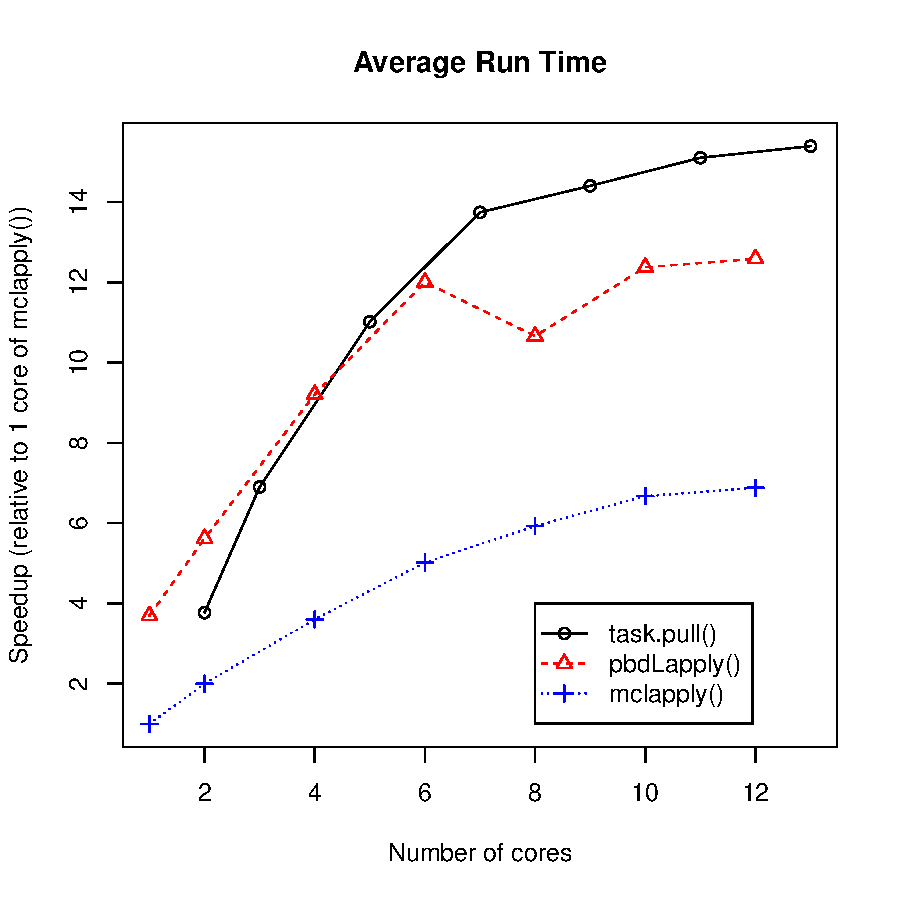
\includegraphics[width=4in]{cubfits-include/figure/avg_run_time}
\caption{Speedup of three different parallelizations.}
\label{fig:speedup}
\end{figure}
